\documentclass[a4paper,titlepage]{book}
\usepackage{frontespizio}
\usepackage[italian]{babel}
\usepackage[utf8]{inputenc}

\usepackage[a4paper, total={6in, 9in}]{geometry}
\usepackage{rotating}


\usepackage{listings}

\lstset{ basicstyle=\small\ttfamily,
numbers=left,
numberstyle=\tiny,
frame=trBL}

\begin{document}
\begin{frontespizio}
\Universita{Verona}
\Dipartimento{Informatica}
\Corso[Laurea]{Informatica}
\Titoletto{Architettura degli Elaboratori}
\Titolo{Relazione Elaborato SIS}

\Candidato[VR363938]{Marco Strambini}
\Candidato[VR353886]{Andrea Olivieri}

\Annoaccademico{2013-2014}
\end{frontespizio}

\tableofcontents



\chapter{Introduzione}

Il progetto è incentrato sulla realizzazione di un circuito che verrà utilizzato in un sistema automobilistico in cui verrà utilizzato come dispositivo per la rilevazione di foratura di pneumatici. È stato realizzato in SIS, partendo da una rappresentazione concettuale grafica, indipendente dall'architettura finale, per poi mappare il prodotto finale in una libreria di componenti chimata \textbf{synch.genlib}.

Di notevole importanza è stata la realizzazione del progetto in higth synthesis level: è stato creato un programma in Excel che simullasse il comportamento del circuito in modo da capire, oltre al funzionamento, la divisione del lavoro tra datapath e fsm.

~

Si è partiti da una due progetti distinti, creando la parte FSM e la parte Datapath, allacciando poi le due parti per creare la FSMD.


\chapter{FSMD}

La FSMD è composta da 14 input (STEERING, RESET, SPEED a 8 bit, ROTDXF, ROTSXF, ROTDXR, ROTSXR) e da 1 output (LIGHT). Quando avviene un malfunzionamento (ossia la foratura di una gomma), monitorato dalla campionatura della velocità e delle rotazioni della ruota anteriore destra, l'output vale 1 e quindi viene segnalato un guasto.

~

Questo componente contiene due sottocomponenti, la FSM che si occupa di tener traccia dello stato attuale del controllo, e del Datapath, che si deve occupare dell'esecuzione dei calcoli e quindi dei confronti della velocità e delle rotazioni.

Il Datapath ha un output direzionato verso la FSM, per generare il segnale di START, mentre la FSM ha un output verso il Datapath per generare il segnale di RESTART; entrambi servono alla campionatura dei controlli.


\begin{figure}[!hb]
\centering
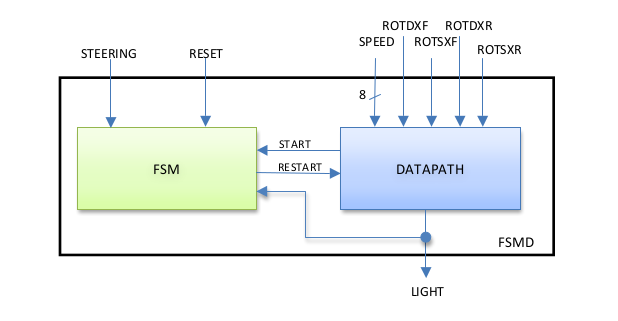
\includegraphics[scale=0.9]{schemi/fsmd.png}
\caption{FSMD}
\end{figure}


\chapter{FSM}

Per capire il funzionamento, bisogna prima analizzare gli inputs e gli outputs:
\begin{itemize}

\item START è un output del DATAPATH: vale 1 se la velocità rilevata è maggiore di 10 $\frac{Km}{h}$;
\item RESET rappresenta un ingresso che serve per resettare il dispositivo: il bit di reset blocca il conteggio dei giri dei pneumatici senza azzerare il numero di giri già calcolato;
\item STEERING rappresenta la fase di sterzo: vale 1 se l'automobile sta sterzando;
\item LIGHT è un output del DATAPATH e vale 1 se almeno uno pneumatico è forato (in base al calcolo del datapath).
~

~

~

~
\item RESTART è l'output della FSM e un input del DATAPATH, vale 1 se, con una velocità maggiore di 10 Km/h, l'automobile è in fase di sterzo;

\end{itemize}

Ora si possono considerare gli stati di questa FSM: sono 4 stati che rappresentano 4 situazioni differenti del sistema di controllo.

PARK è lo stato iniziale della FSM. L'automobile si trova in questo stato quando la sua velocità è inferiore a 10 Km/h o quando riceve il segnale di reset. In questo stato non viene incrementato il numero di giri dei pneumatici in quanto la velocità dell'automobile è troppo bassa (come da specifiche).
 
COUNT è lo stato in cui si avviano i conteggi del numero di giri di ogni pneumatico. Questo stato si può raggiungere quando START vale 1 e gli altri ingressi sono posti a 0.

STOP\_COUNT è lo stato in cui si interrompe il conteggio del giri di ogni pneumatico in quanto l'automobile è in fase di sterzo. Questo stato è
raggiungibile da tutti gli altri stati se e solo se START e STEERING valgono 1, mentre gli altri ingressi sono posti a 0. In questo caso l'automobile ha una velocità maggiore di 10 Km/h ed è in fase di sterzo.

LIGHT è lo stato in cui si accende la spia che indica la foratura di uno pneumatico. Questo stato è raggiungibile dagli altri se e solo START e LIGHT valgono 1 e RESET vale 0.


\begin{figure}[!hb]
\centering
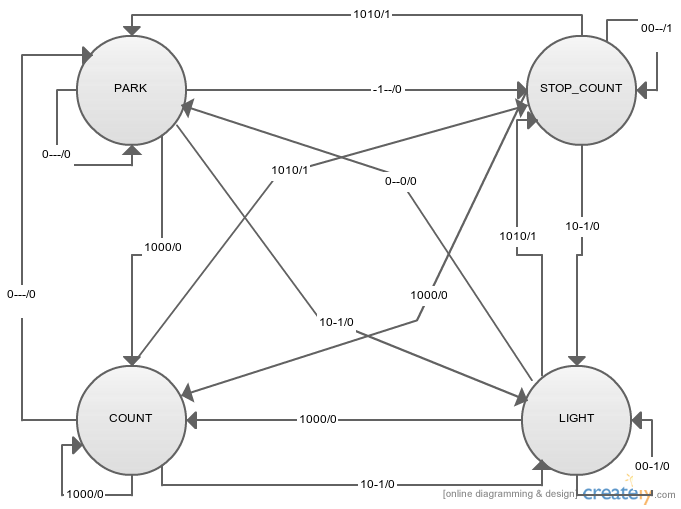
\includegraphics[scale=0.5]{schemi/fsm.png}
\caption{FSM}
\end{figure}



\chapter{Datapath}

Per capire il funzionamento, bisogna prima analizzare gli inputs e gli outputs:
\begin{itemize}

\item RESTART è l'output della FSM: vale 1 se, con una velocità maggiore di 10 Km/h, l'automobile è in fase di sterzo;
\item SPEED rappresenta la velocità dell'automobile: è espressa in modulo a 8 bit e può assumere valori da 0 a 255;
\item ROTDXF rappresenta la ruota anteriore destra: vale 1 se la ruota fa un giro completo;
\item ROTSXF rappresenta la ruota anteriore sinistra: vale 1 se la ruota fa un giro completo;
\item ROTDXR rappresenta la ruota posteriore destra: vale 1 se la ruota fa un giro completo;
\item ROTSXR rappresenta la ruota posteriore sinistra: vale 1 se la ruota fa un giro completo.
\item START è un output del DATAPATH e un input della FSM: vale 1 se la velocità dell'automobile risulta maggiore di 10 Km/h;
\item LIGHT è un output del DATAPATH e un input della FSM, è anche l'output del circuito sequenziale; vale 1 se è stato riscontrato che almeno uno pneumatico ha effettuato un numero di giri troppo basso per poter sembrare non forato.
\end{itemize}

\begin{figure}[!hb]
\centering
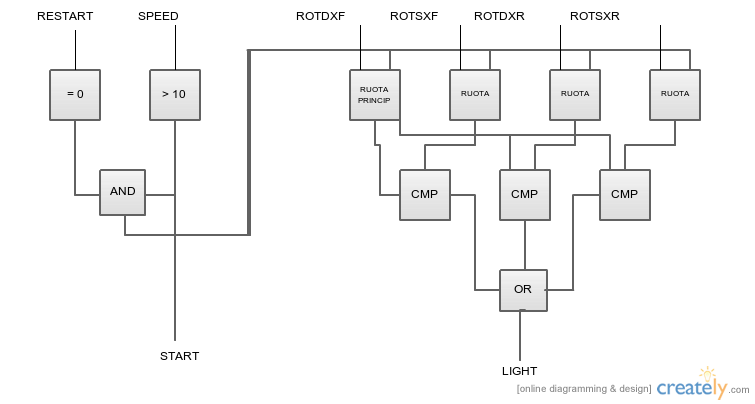
\includegraphics[scale=0.45]{schemi/datapath.png}
\caption{Datapath}
\end{figure}


\section{Composizione}

Il DATAPATH è costituito dai seguenti file con estensione .blif: velox.blif signal.blif ruota\_principale.blif ruota.blif diff.blif or3.blif




\subsection{velox.blif}
Restituisce 1 se e solo se gli 8 bit di input rappresentano un valore maggiore di 10. In questo caso l'output di velocita.blif costituisce l'output START del DATAPATH. Esso indica che la velocità dell'automobile è superiore a 10 Km/h.



\begin{figure}[!hb]
\centering
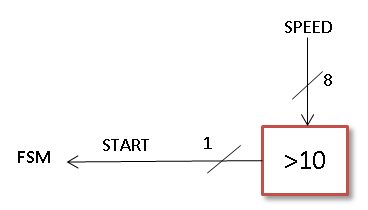
\includegraphics[scale=0.5]{schemi/velox.png}
\caption{Velox}
\end{figure}


\subsection{signal.blif}
Riceve come input i valori di RESTART (1 bit) e SPEED (8 bit). Se il bit di RESTART vale 0 e la velocità è superiore a 10 km/h, allora restituisce 1, altrimenti restituisce 0.



\begin{figure}[!hb]
\centering
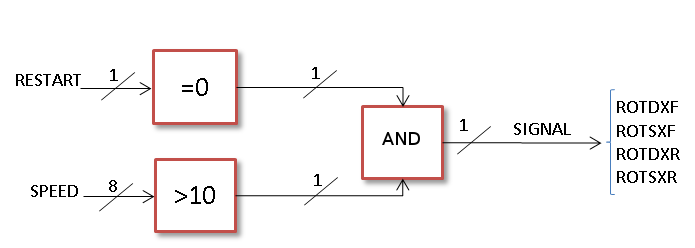
\includegraphics[scale=0.5]{schemi/signal.png}
\caption{Signal}
\end{figure}


\subsection{ruota\_principale.blif}
Riceve in input il bit restituito dal file segnale.blif SIGNAL e ROTDXF.  Se SIGNAL vale 0, il multiplexer seleziona la costante 0. Questo caso si verifica quando  l'automobile si trova in fase di sterzo oppure ha una velocità troppo bassa. In queste due  condizioni il dispositivo non incrementa il numero di giri del pneumatico, ma continua a  sommare 0 al numero che rappresenta i giri del pneumatico, il quale rimane invariato.  Altrimenti, se SIGNAL vale 1, il multiplexer seleziona il valore della ruota, che potrebbe  essere 0, se la ruota non ha effettuato un giro completo, oppure 1, se la ruota ha  effettuato un giro completo.  Il registro, inizializzato a 0, memorizza un numero a 6 bit che rappresenta il numero di giri  completi effettuati dalla ruota.  Il contatore prende in input il valore contenuto dal registro e la costante appena  selezionata dal multiplexer, sommando al primo la costante e restituendo un numero che  potrebbe essere invariato, se è stato sommato 0, oppure incrementato di 1, se è stato  sommato 1.  A questo punto il multiplexer deve selezionare quale valore salvare nel registro: il numero  restituito dal contatore oppure una costante 0 a 6 bit, la quale serve per azzerare il  contenuto del registro.  Nel frattempo un altro componente controlla se il numero appena restituito dal contatore  sia uguale a 50. In questo caso il multiplexer seleziona la costante 0 a 6 bit e la restituisce  come output, permettendo al registro di salvarla al suo interno e azzerarsi. Altrimenti, se il  numero è minore di 50, il multiplexer seleziona il numero restituito dal contatore, il quale si  salverà nel registro.  ruota\_princ.blif restituisce in output un bit, il quale vale 0 se il numero di giri del  pneumatico è inferiore a 50, altrimenti vale 1 se il pneumatico ha effettuato 50 giri.



\begin{figure}[!hb]
\centering
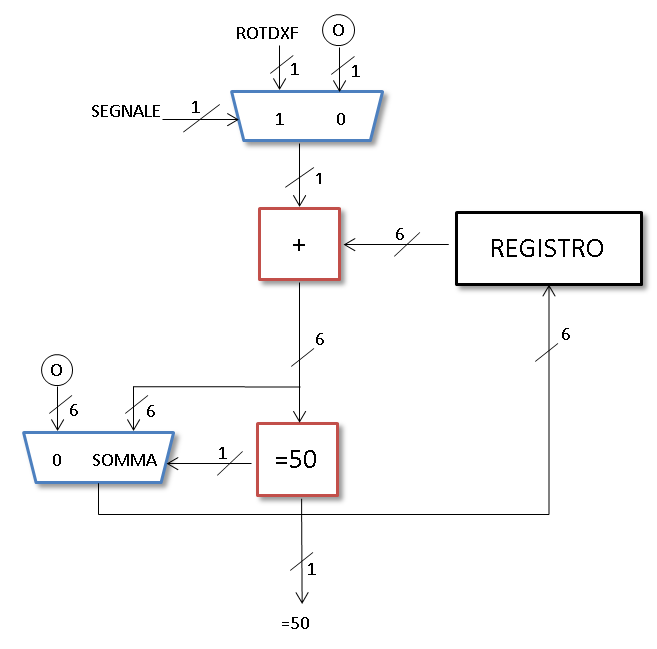
\includegraphics[scale=0.5]{schemi/ruota_principale.png}
\caption{Ruota principale}
\end{figure}



\subsection{ruota.blif}

La struttura di questo file è analoga a quella di ruota\_princ.blif, ma presenta qualche lieve  differenza.  Anzitutto presenta un input in più, cioè un segnale UG50 che corrisponde all'output della  ruota anteriore destra e vale 1 se quest'ultima ha raggiunto i 50 giri, altrimenti vale 0. Il  multiplexer dovrà leggere ogni volta il valore di questo bit per decidere quale valore  restituire al registro perché quest'ultimo possa memorizzarlo al suo interno.  Inoltre ruota.blif restituisce come output il valore del registro appena incrementato dal  contatore.  Infine, il contatore utilizzato in questo caso è implementato in contatore6bis.blif. Esso  realizza un contatore analogo a contatore6.blif ma conta fino a 60, azzerandosi  successivamente. Questo permette di continuare a contare i giri delle ruote anteriore  sinistra e posteriore destra e sinistra anche quando la ruota di riferimento per qualche  motivo gira più lentamente senza essere bucata. I confronti sui giri dei pneumatici si  avviano quando la ruota di riferimento arriva a 50 giri. Per cui se il pneumatico di  riferimento effettua in 100 metri 45 giri, mentre gli altri ne effettuano 50, il confronto  avverrà quando il primo sarà arrivato a 50 giri e gli altri a 55 giri, supponendo che abbiano  girato sempre correttamente. La differenza tra 55 e 50 è infatti minore del 20\%.  



\begin{figure}[!hb]
\centering
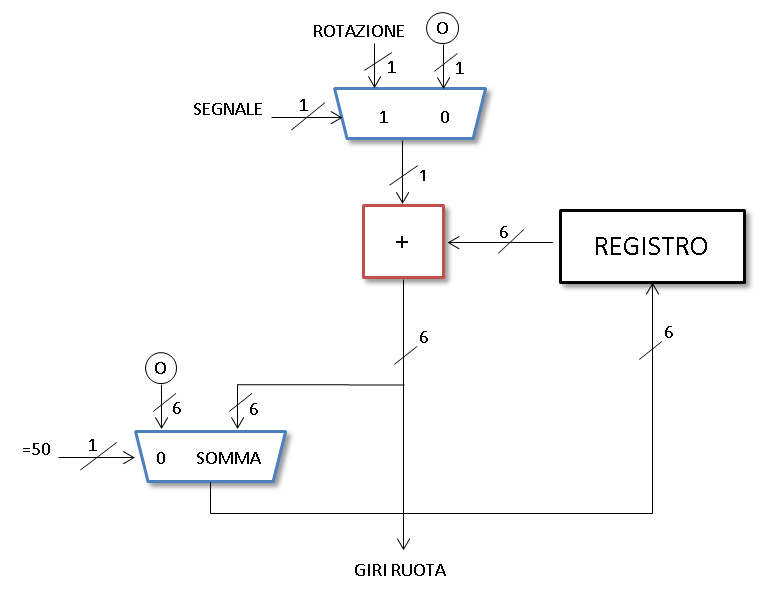
\includegraphics[scale=0.5]{schemi/ruota.png}
\caption{Ruota}
\end{figure}


\subsection{diff.blif}

Questo file di occupa di controllare che la differenza tra il numero di giri della ruota di  riferimento, cioè quella anteriore destra, e ognuna delle altre tre ruote sia inferiore al 20\%.  differenza.blif riceve in input un segnale S, che indica se la ruota anteriore destra ha  effettuato 50 giri, e un numero a 6 bit, che rappresenta il numero di giri effettuato dalla  ruota che deve essere confrontata con quella di riferimento. Il confronto ha senso solo se  il segnale S vale 1  Quindi, se la differenza tra 50, cioè il numero di giri del pneumatico anteriore destro, e il  numero di giri del pneumatico da confrontare è inferiore al 20\%, allora l'uscita di  differenza.blif vale 0. In caso contrario, per cui di differenza superiore al 20\%, l'uscita vale  1.


\subsection{or3.blif}

Rappresenta un componente or a 3 bit. Questo ha uscita zero se e solo se tutti e 3 i bit in  entrata valgono 0.  or3.blif riceve in input 3 bit, ognuno dei quali rappresenta l'esito di un confronto sul  numero di giri tra la ruota “principale” e ciascuna delle altre 3 ruote.  Se tutte le ruote, compresa quella di riferimento, hanno girato correttamente, gli input di  OR3 saranno 3 zeri e l'uscita avrà valore 0.  Altrimenti, se almeno una ruota non ha girato correttamente, almeno un input di OR3 sarà  1 e quindi anche la sua uscita avrà valore 1.  L'output di OR3 è LIGHT. Questo è un output del DATAPATH e anche l'unico della FSMD.  Esso costituisce inoltre un input per la FSM.  Se LIGHT vale 1, significa che il dispositivo ha rilevato un problema sul numero di giri dei  pneumatici su una distanza pari a 100 metri.



\begin{figure}[!hb]
\centering
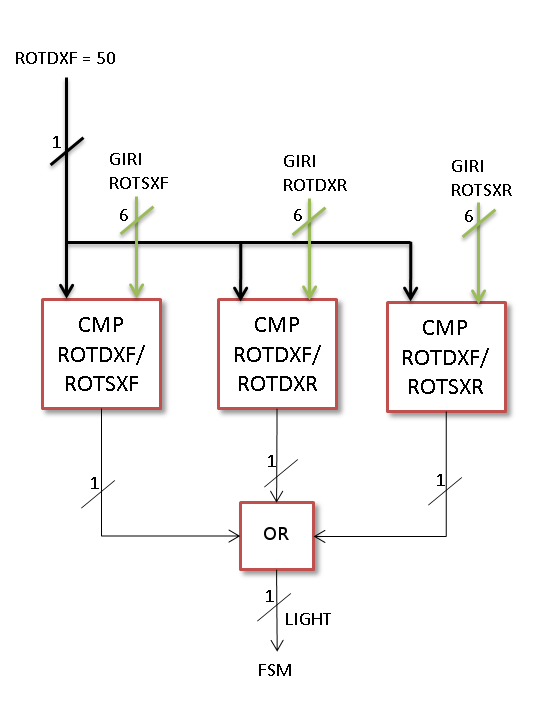
\includegraphics[scale=0.5]{schemi/diff_or3.png}
\caption{Diff e or3}
\end{figure}

\chapter{Mapping e ottimizzazione}

È stato deciso di ottimizzare il circuito finale (FSMD.blif) in modo da poter lavorare su un unico file ed eseguire uno script che potesse minimizzare il numero di letterali il più possibile.
Lo script ha il seguente path: \textit{FSMD/script\_ottimizzazione.script}

La situazione iniziale era questa:

\begin{lstlisting}
sis> read_blif FSMD.blif
Warning: network `FSMD', node "STEERING" does not fanout
Warning: network `FSMD', node "RESET" does not fanout
Warning: network `FSMD', node "START" does not fanout
sis> print_stats
FSMD          	pi=14	po= 1	nodes= 91	latches=24
lits(sop)=9471
sis>
\end{lstlisting}


Dopo aver eseguito lo script che genera la FSMD mappata (gen\_fsmd.script) è stato ottenuto questo:

\begin{lstlisting}
sis> source gen_fsmd.script
Warning: network `FSMD', node "STEERING" does not fanout
Warning: network `FSMD', node "RESET" does not fanout
Warning: network `FSMD', node "START" does not fanout
FSMD          	pi=14	po= 1	nodes= 59	latches=24
lits(sop)= 413
WARNING: uses as primary input drive the value (0.20,0.20)
WARNING: uses as primary input arrival the value (0.00,0.00)
WARNING: uses as primary input max load limit the value (999.00)
WARNING: uses as primary output required the value (0.00,0.00)
WARNING: uses as primary output load the value 1.00
Total Area		= 6504.00
Gate Count		= 170
Buffer Count		= 5
Inverter Count 		= 32
Most Negative Slack	= -27.00
Sum of Negative Slacks	= -588.00
Number of Critical PO	= 25
[1837]     or2_comb        32.00	
[1304]     aoi12_comb      32.00	
[1389]     invand_comb     32.00	
[2241]     or4_comb        48.00	
[720]      aoi12_comb      32.00	
[1848]     nand3_comb      32.00	
[1765]     invand_comb     32.00	
[1842]     nand2_comb      24.00	
[1846]     or3_comb        40.00	
[1380]     nor2_comb       24.00	
[1850]     oai12_comb      32.00	
[1851]     invor_comb      32.00	
[1273]     invand_comb     32.00	
[1379]     nor2_comb       24.00	
[1272]     aoi12_comb      32.00	
[2020]     oai22_comb      40.00	
[1839]     inv_comb        16.00	
[1844]     inv_comb        16.00	
[1853]     or3_comb        40.00	
[1841]     inv_comb        16.00	
[1843]     inv_comb        16.00	
[1387]     nor3_comb       32.00	
[2576]     oai12_comb      32.00	
[1270]     nor2_comb       24.00	
[1855]     oai12_comb      32.00	
[1383]     nor3_comb       32.00	
[1783]     nor2_comb       24.00	
[1773]     aoi12_comb      32.00	
[2014]     inv_comb        16.00	
[2017]     oai12_comb      32.00	
[1860]     nand3_comb      32.00	
ROT1_O5MUX6 dff_reset_re    104.00	
[2019]     inv_comb        16.00	
ROT1_O4MUX6 dff_reset_re    104.00	
[1375]     nor2_comb       24.00	
[1292]     aoi12_comb      32.00	
ROT1_O3MUX6 dff_reset_re    104.00	
[2436]     oai12_comb      32.00	
[2698]     and3_comb       40.00	
ROT1_O2MUX6 dff_re          88.00	
[2021]     inv_comb        16.00	
ROT1_O1MUX6 dff_reset_re    104.00	
[2700]     inv_comb        16.00	
[2231]     dff_re          88.00	
[1698]     aoi12_comb      32.00	
[1863]     inv_comb        16.00	
[2355]     nand3_comb      32.00	
[1869]     nand3_comb      32.00	
[1870]     invor_comb      32.00	
[1875]     nand3_comb      32.00	
[1369]     nor3_comb       32.00	
[1695]     aoi12_comb      32.00	
[1295]     and2_comb       32.00	
O5MUX6     dff_reset_re    104.00	
[1873]     inv_comb        16.00	
[1871]     inv_comb        16.00	
[1862]     inv_comb        16.00	
[2546]     oai12_comb      32.00	
[1276]     and2_comb       32.00	
[1879]     oai22_comb      40.00	
[2540]     oai12_comb      32.00	
[1878]     nand2_comb      24.00	
[1880]     oai12_comb      32.00	
[1361]     nor2_comb       24.00	
[2532]     oai12_comb      32.00	
[2072]     inv_comb        16.00	
[1881]     oai12_comb      32.00	
[2064]     inv_comb        16.00	
O4MUX6     dff_reset_re    104.00	
[2067]     inv_comb        16.00	
O3MUX6     dff_reset_re    104.00	
O2MUX6     dff_reset_re    104.00	
[2329]     inv_comb        16.00	
[1647]     aoi12_comb      32.00	
[1883]     oai12_comb      32.00	
O1MUX6     dff_reset_re    104.00	
[1884]     nand2_comb      24.00	
[1297]     aoi12_comb      32.00	
[1296]     nor2_comb       24.00	
[2706]     nor3_comb       32.00	
O0MUX6     dff_re          88.00	
[1608]     aoi12_comb      32.00	
[1887]     inv_comb        16.00	
[2349]     nand3_comb      32.00	
[1893]     nand3_comb      32.00	
[1894]     invor_comb      32.00	
[1899]     nand3_comb      32.00	
[1354]     nor3_comb       32.00	
[1605]     aoi12_comb      32.00	
[1298]     and2_comb       32.00	
[461]      dff_reset_re    104.00	
[1897]     inv_comb        16.00	
[1895]     inv_comb        16.00	
[1886]     inv_comb        16.00	
[2524]     oai12_comb      32.00	
[1282]     and2_comb       32.00	
[1903]     oai22_comb      40.00	
[2518]     oai12_comb      32.00	
[1902]     nand2_comb      24.00	
[1904]     oai12_comb      32.00	
[1346]     nor2_comb       24.00	
[2510]     oai12_comb      32.00	
[2129]     inv_comb        16.00	
[1905]     oai12_comb      32.00	
[2121]     inv_comb        16.00	
[462]      dff_reset_re    104.00	
[2124]     inv_comb        16.00	
[463]      dff_reset_re    104.00	
[464]      dff_reset_re    104.00	
[2337]     inv_comb        16.00	
[1557]     aoi12_comb      32.00	
[1907]     oai12_comb      32.00	
[465]      dff_reset_re    104.00	
[1908]     nand2_comb      24.00	
[1300]     aoi12_comb      32.00	
[1299]     nor2_comb       24.00	
[2712]     nor3_comb       32.00	
[466]      dff_re          88.00	
[1518]     aoi12_comb      32.00	
[1911]     inv_comb        16.00	
[2352]     nand3_comb      32.00	
[1917]     nand3_comb      32.00	
[1918]     invor_comb      32.00	
[1923]     nand3_comb      32.00	
[1339]     nor3_comb       32.00	
[1515]     aoi12_comb      32.00	
[1301]     and2_comb       32.00	
[487]      dff_reset_re    104.00	
[1921]     inv_comb        16.00	
[1919]     inv_comb        16.00	
[1910]     inv_comb        16.00	
[2502]     oai12_comb      32.00	
[1288]     and2_comb       32.00	
[1927]     oai22_comb      40.00	
[2496]     oai12_comb      32.00	
[1926]     nand2_comb      24.00	
[1928]     oai12_comb      32.00	
[1331]     nor2_comb       24.00	
[2488]     oai12_comb      32.00	
[2186]     inv_comb        16.00	
[1929]     oai12_comb      32.00	
[2178]     inv_comb        16.00	
[488]      dff_reset_re    104.00	
[2181]     inv_comb        16.00	
[489]      dff_reset_re    104.00	
[490]      dff_reset_re    104.00	
[2321]     inv_comb        16.00	
[1467]     aoi12_comb      32.00	
[1931]     oai12_comb      32.00	
[491]      dff_reset_re    104.00	
[1932]     nand2_comb      24.00	
[1303]     aoi12_comb      32.00	
[1302]     nor2_comb       24.00	
[2718]     nor3_comb       32.00	
[492]      dff_re          88.00	
[1940]     nand3_comb      32.00	
[1269]     and2_comb       32.00	
[2382]     oai12_comb      32.00	
[2482]     nand3_comb      32.00	
[1311]     aoi12_comb      32.00	
[1267]     and2_comb       32.00	
[2378]     oai12_comb      32.00	
[2474]     nand3_comb      32.00	
[1309]     aoi12_comb      32.00	
[1268]     and2_comb       32.00	
[2380]     oai12_comb      32.00	
[2478]     nand3_comb      32.00	
[1310]     aoi12_comb      32.00	
[1260]     nor4_comb       40.00	
{LIGHT}    nor2_comb       24.00
sis>
\end{lstlisting}

Quindi è stato ottimizzato tantissimo il numero di letterali (da 9471 a 413) e quindi mappando ed ottimizzando per area (map -m 0) è stato generato un circuito sicuramente più piccolo di quello che sarebbe stato generato senza lo script di ottimizzazione.

Lo script di ottimizzazione è il seguente:

\begin{lstlisting}
sweep			#Esegue l'operazione di sweep;
eliminate 20		#Esegue l'operazione di eliminazione 
			#rimuovendo i nodi tali che la loro 
			#rimozione non aumenti il numero di 
			#letterali di una quantita' superiore 
			#a ``n''

fx			#Esegue l'operazione di estrazione;
full_simplify		#Esegue l'operazione di semplificazione su ogni
			#nodo della rete;

eliminate 1
resub 			#Esegue l'operazione di scomposizione dei nodi
			#indicati nella lista. Se la lista non viene 
			#specificata, la sostituzione viene eseguita 
			#per tutti i nodi della rete. 

resub 
eliminate 2
full_simplify
fx
fx
fx
sweep
resub 
resub 
full_simplify
eliminate 1
eliminate 2
full_simplify

print_stats		#stampa le statistiche del risultato

\end{lstlisting}


\end{document}
